\vspace{-10ex}%
\rule{\textwidth}{0.3pt}
\vspace{5ex}

\textit{
This chapter will introduce the reader to the problem formulation and the underlying principles taken into account. The principle of radio communication and the important steps involved in developing a new product prototype will be presented. Basic information about the communication and programming will also be presented. 
}
\vspace{5ex}


\section{PCB}
Good characteristics of the circuit the system will be produced on a four-layer \gls{pcb}. This has a lot of advantages over a standard two-layer board. The four-layer design will have a top layer where all the components will be placed, a bottom layer with extra room for tracing tracks and having another ground polygon. The two inner layers consist of a power plane and a ground layer. Benefits of this are both easier connectability and also as a good way of making the circuit more resistant to high-frequency noise between the traces on the top and bottom layer. 



\section{Radio Frequency}
Radio frequencies are a set of frequencies that are used for transceiving and receiving data wirelessly. Radio frequencies begin at one end of the spectrum where the frequencies are about 100Hz. It contains all the frequencies up to 300Ghz. Radio frequencies are divided into different bands, all with different characteristics and areas of implementation. A frequency spectrum is provided in \autoref{fig:full_freq_band}.

\begin{figure}[H] 
    \centering 
    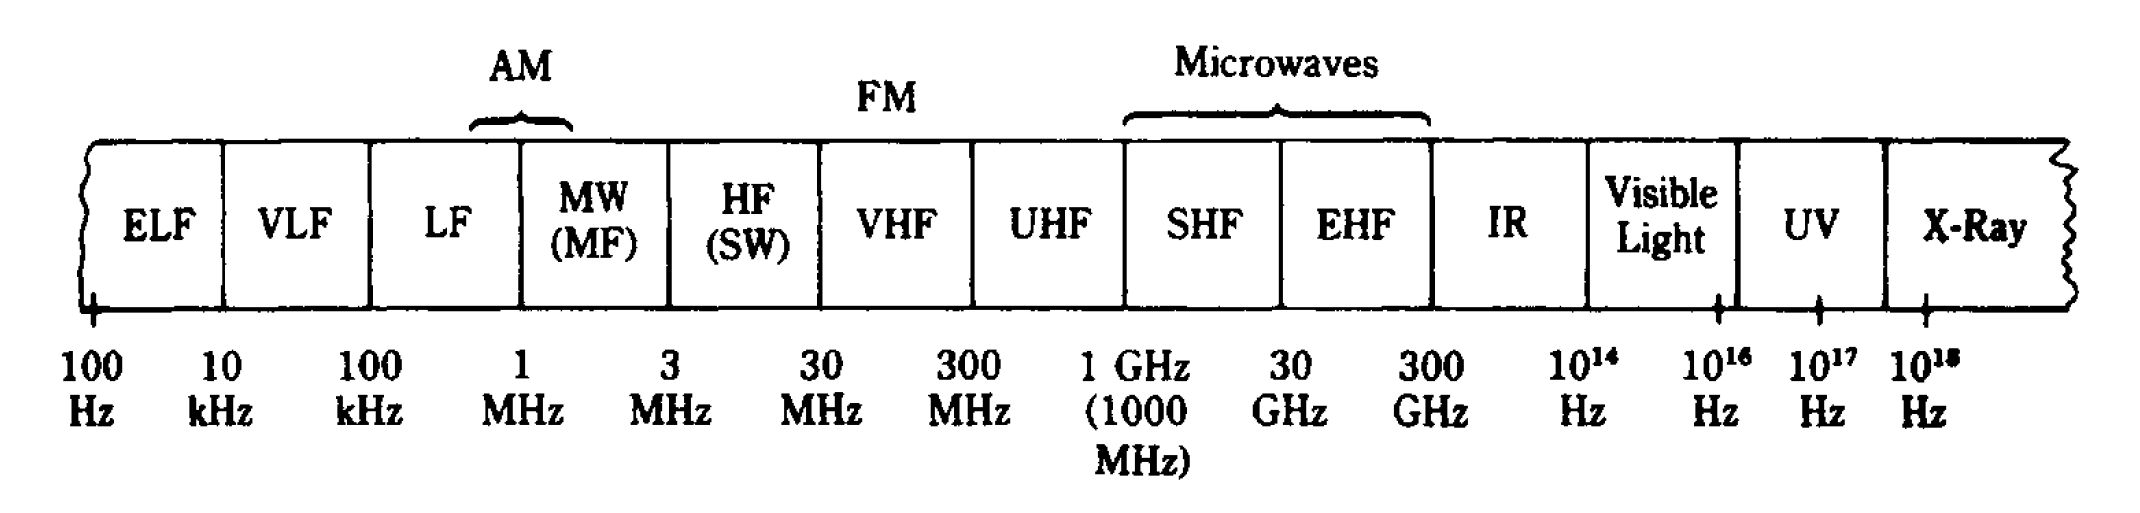
\includegraphics[width=.8\linewidth]{Figures/Full_frequency_band} 
    \captionsource{Electromagnitical frequencies}{RF Circuit Design \cite{rf_circut_design}}
    \label{fig:full_freq_band} 
\end{figure} 

\section{Problems}
Designing a circuit for radio transmission is an advanced and complex procedure. 
The high frequencies introduce a lot of interesting phenomena that need to be considered when constructing a circuit in these frequencies. 
When designing a circuit for \gls{rf}, components and traces on the \gls{pcb} behaves in a different way and takes on different characteristics than an equal system at lower frequencies. 
Some of the challenges that arise are described in Secrets of RF Circuit Design \cite{secrets_of_rf}. 
Stray capacitance is one of the phenomena that arise when handling \gls{rf}. 
Between conductors, conductors to ground and between components a small capacitance occurs when dealing with \gls{rf}.
\newline
Another phenomenon that introduces is the so-called skin effect, where the "skin" part comes from the physical phenomena that are happening. When the frequencies rise the resistance in a conductors core increases with it. As current choose the path of least resistance and will therefore in higher frequencies flow only on the outside most part of a component. A visual explanation of this can be seen in \autoref{skin_effect}.
\newline
%To ensure a good radio signal some criteria need to be fulfilled. 
%Radio frequencies do many things to a board, these problems and appearances have to be evaluated and considered.  Some of these problems is described in High speed digital design by %Johnson \& Graham \cite{high_speed_digital}.
The output signal from the radio transceiver is matched at 50 ohms and this has to be matched with the output stage components. These components commonly is a network of inductors and capacitors. This matching network is described later in this section. 
From different types of radio signal transceiver, the type used in this case is determined by the radio \gls{ic}'s manufacturer. \cite{si4460}
%High-speed Digital design – Johnson & Graham

%"Secrets of RF Circuit Design"
\subsection{Class E amplifier}
The \gls{cle} amplifier type used here uses switching type of amplification to increase efficiency and reduce power loss. 
The most interesting part of \gls{cle} is the fact that up to ideal power efficiency can be achieved by constructing this type. \cite{class_e_new}
%Class E makes use f

\subsection{Chebychev Filter}
The Chebyshev type of filter is special in the fact that it has a steep fall rate and a high \emph{Q}. The \emph{Q} factor is commonly used in filter design as a function of the length of the stopband through the whole passband.
This makes it very suited for radio designs.




\subsection{Radio antenna filter}
Stating in the datasheet to the radio \gls{ic} the rough design aspects are defined. The Chebyshev filter is recommended for this radio for its good characteristics. With a high Q value the steeper the slope is in the stop-band region.



\section{SPI}
\gls{spi} communication is used to communicate between the \gls{mcu} and other \gls{ic}'s on a circuit board.\gls{spi} uses four wires to communicate and additional one wire for each extra \gls{ic} that is connected. The transmission works in a synchronous serial manner where each bit is sent one at the time synchronous to a supplied clock signal. Different types of \gls{spi} connections exist but with the most common being the four-wire serial bus. Here SCL, SDO, SDI, and SS is used. \cite{pic_spi} 

\begin{itemize}[noitemsep]
    \item SCL  -      Serial CLock, a clock is supplied to synchronize the data transmissions.
    \item SDO -     Serial Data Out, Data is sent from this port.
    \item SDI  -     Serial Data In, Data is transmitted to this port.
    \item SS    -     Slave Select, Selects a device for communication.
\end{itemize}
 
Eight bits are sent together to form a package of one byte. Four different modes are available when communicating through \gls{spi}. These modes determine which type of clock signal provided and how the data is sampled in the devices. Two different types of clock-signal, one where the clock is pulled high when idle and the other one pulled low when idle. This is often called in the registers as; CPOL. 
The other mode selects the timing of data bits relative to the clock signal. Data is sampled either when the clock signal goes high or in the middle of a clock pulse. CPHA is the often the name of this selection. This concludes the different modes. A visual explanation of \gls{spi} communication is provided in \autoref{fig:SPI_timing}. 


\begin{figure}[H]
    \centering
    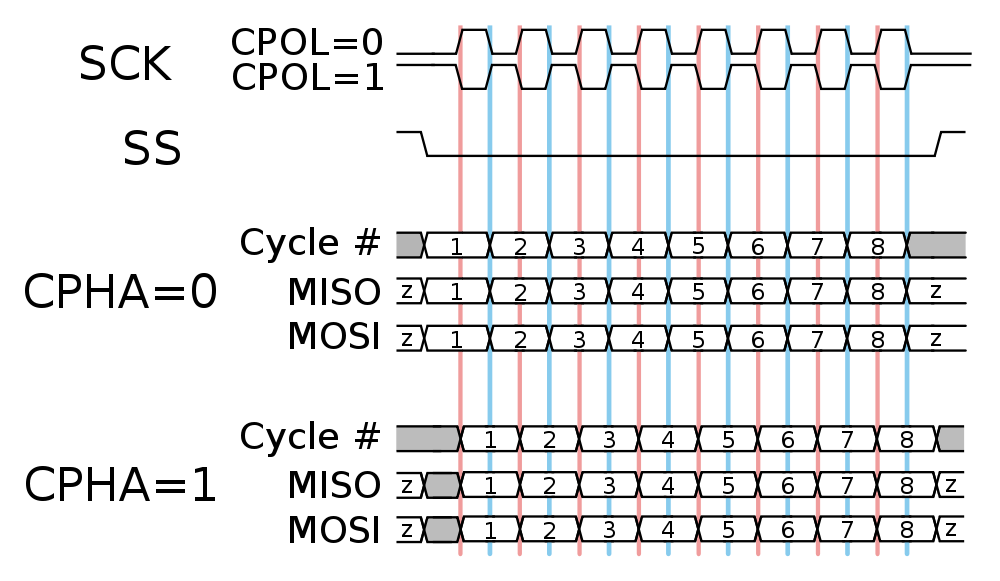
\includegraphics[width=.8\linewidth]{Figures/SPI_timing}
    \captionsource{Timing and modes for a transmission over \gls{spi}}{\url{https://commons.wikimedia.org/wiki/File:SPI_timing_diagram.svg}}
    \label{fig:SPI_timing}
\end{figure}


The interface uses one master device and multiple slaves. The master device handles the communication and supplies the selection of slaves. To enable a connection and choose which slave is used an individual slave select must be present. When set, only the chosen slave device is able to communicate.

From the \gls{mcu}'s datasheet the following diagram show in \autoref{fig:PIC_SPI} how the connection works when connection several slave devices.

\begin{figure}[H]
    \centering
    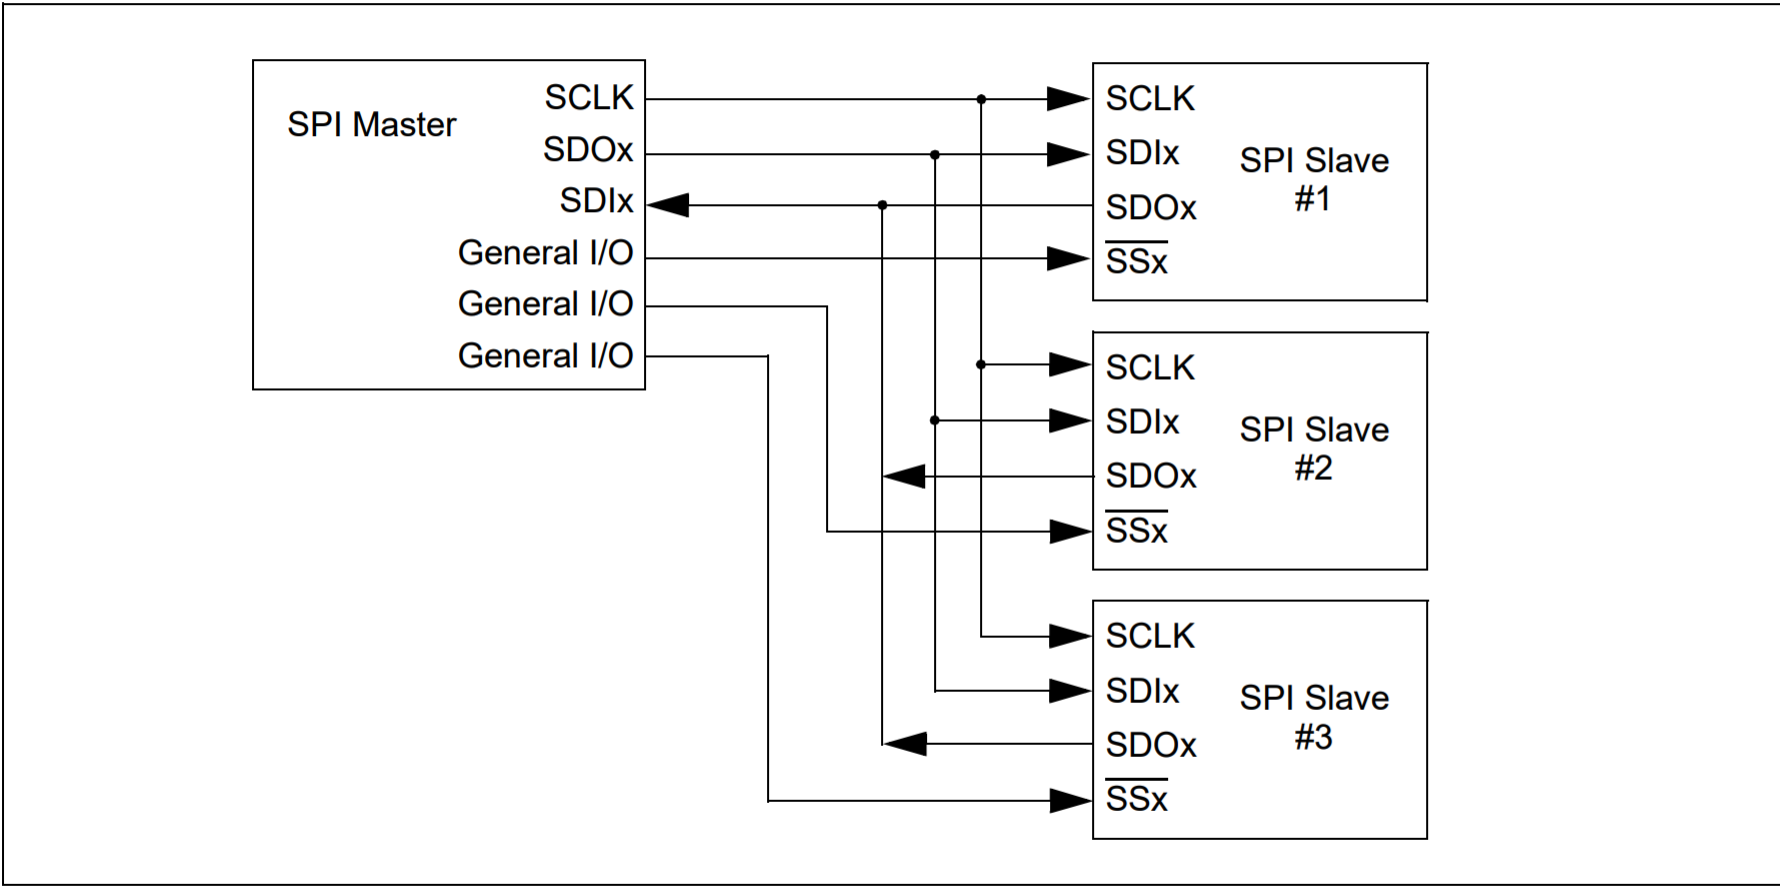
\includegraphics[width=.8\linewidth]{Figures/PIC_SPI}
    \captionsource{SPI master and multiple slave connections}{\url{http://ww1.microchip.com/downloads/en/DeviceDoc/40001412G.pdf}}
    \label{fig:PIC_SPI}
\end{figure}
Data is sent out from the \gls{mcu} at the SDO wire and at the other end connected to the SDI pin of a receiving device. 


\section{I$^2$C}
A more advanced type of communication is \gls{i2c}. \gls{i2c} is more often used in larger circuits or when the distances are longer. The \gls{i2c} interface uses pull-up resistors to set the idle state of the signals high. Different speeds require different types of resistors, with the higher resistors not able to handle faster transfer speeds but draw less power when transmitting data.  

 